% Intended LaTeX compiler: pdflatex
\documentclass[11pt]{article}
\usepackage[utf8]{inputenc}
\usepackage[T1]{fontenc}
\usepackage{graphicx}
\usepackage{longtable}
\usepackage{wrapfig}
\usepackage{rotating}
\usepackage[normalem]{ulem}
\usepackage{amsmath}
\usepackage{amssymb}
\usepackage{capt-of}
\usepackage{hyperref}
\usepackage{graphicx} \graphicspath{{./src/}}
\author{Antonio Petrillo}
\date{}
\title{Documentazione progetto basi di dati}
\hypersetup{
 pdfauthor={Antonio Petrillo},
 pdftitle={Documentazione progetto basi di dati},
 pdfkeywords={},
 pdfsubject={},
 pdfcreator={Emacs 29.0.91 (Org mode 9.6.1)}, 
 pdflang={English}}
\begin{document}

\maketitle
\setcounter{tocdepth}{2}
\tableofcontents

\section*{Traccia originale}
\label{sec:org8ab949f}
Scenario: l’organizzazione di un cantiere edile Attori:
\begin{itemize}
\item Amministratore del sistema: che ha possibilità di modificare tutto il database
\item Capocantiere: che gestisce il cantiere di cui è responsabile
\end{itemize}
Bisogna andare a gestire l’organizzazione di un certo numero di cantieri. L’apertura di un cantiere è fatta dall’amministratore del sistema che poi ne demanda la gestione al Capocantiere.
Il capocantiere dovrà tenere traccia di:
\begin{itemize}
\item Gli operai che lavorano nel cantiere, definendo per ognuno un ruolo all’interno del cantiere
\item Aree del cantiere: ad esempio un cantiere può essere diviso in 3 aree, una zona da adibire
\end{itemize}
a verde pubblico, una da adibire a zona residenziale, un’altra da adibire a servizi pubblici.
\begin{itemize}
\item Ogni area del cantiere ha un operaio che ne è responsabile
\end{itemize}
Si definisca anche un ruolo “operatore”, il quale ha il compito di piazzare dei sensori all’interno del cantiere. Questi sensori devono monitorare il livello di rumore in una particolare area del cantiere, e eventuali fughe di gas all’interno dell’area. Ogni area possiede una sola coppia di sensori.
Il capocantiere deve essere in grado di leggere e filtrare i dati dei sensori. I dati dei sensori per ogni area e per ogni cantiere possono essere inseriti dal capocantiere o dall’amministratore. Si definisca una soglia al di sopra della quale viene lanciato un allarme (rumore troppo alto e quantità di gas molto elevata). Il capocantiere e l’amministratore possono modificare questa soglia.
\section*{Descrizione}
\label{sec:orgae0d11a}
Progettazione di una base dati atta a contenere informazioni di cantieri edili.

\textbf{Un cantiere é caratterizzato nel seguente modo:}
\begin{itemize}
\item \textbf{Amministratore}, avvia il progetto di un cantiere.
Esso puó aprire un nuovo cantiere e delegarne il controllo ad un \emph{capocantiere}, inoltre puó modificare la \emph{soglia} al di sopra delle quale i \emph{sensori} lanciano un allarme
\item \textbf{Capocantiere}, gestisce un particolare cantiere.
Il suo compito principale é quello di leggere i \emph{sensori} del cantiere a cui é assegnato, inoltre anche esso puó modificare la \emph{soglia} di allarme dei \emph{sensori}.
\item \textbf{Cantiere}.
Ogni cantiere é suddiviso in piú \emph{aree}.
\item \textbf{Area}.
Area di un determinato \textbf{cantiere}.
Ogni area possiede due \textbf{sensori}.
\item \textbf{Sensore}.
Sensore installato in una particolare \textbf{area} di un \textbf{cantiere}.
Ogni sensore viene installato da un \textbf{operatore}.
Ogni sensore possiede una soglia al di sopra della quale genera un allarme.
Ve ne sono di due tipi:
\begin{itemize}
\item Monitorarizzazione del \textbf{rumore}
\item Monitorarizzazione del \textbf{gas}
\end{itemize}
\item \textbf{Operaio}.
Impiegato del cantiere.
\end{itemize}
\section*{Progettazione Concettuale}
\label{sec:orgb951e4a}
\subsection*{Diagramma concettuale}
\label{sec:org8cb1f65}
\(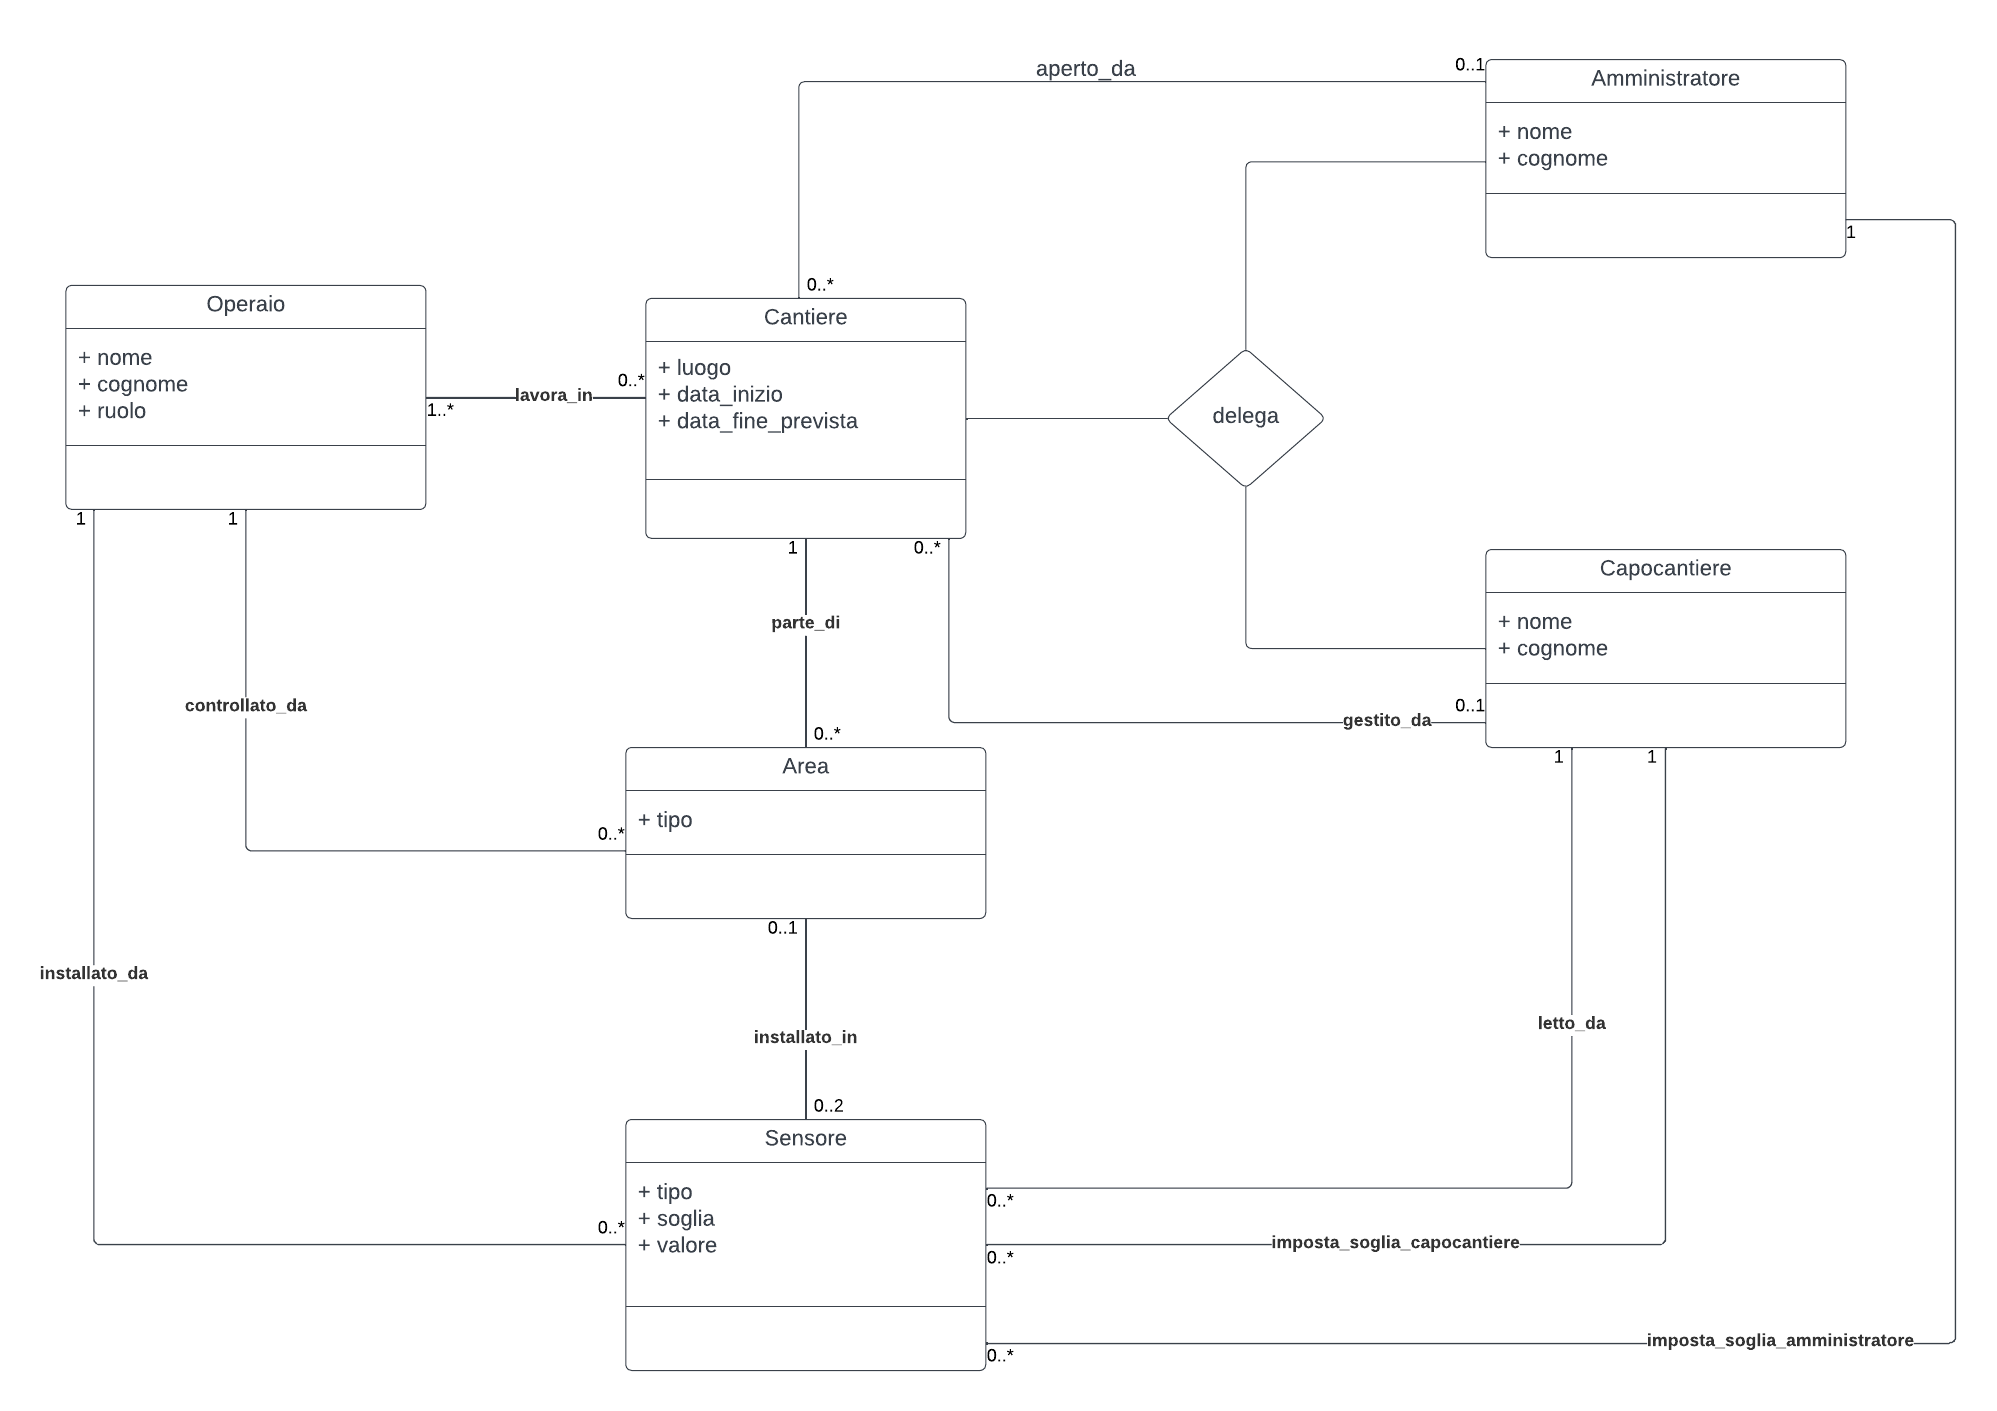
\includegraphics[scale=0.5]{cantiereconcettuale.png}\)
\subsection*{Ristrutturazione}
\label{sec:orgab3802d}
\subsubsection*{Rimozione ridondanze}
\label{sec:org22c2c36}
Viene esplicitamente richiesto che un \textbf{Sensore} abbia una soglia impostabile da parte dell'amministratore e del capocantiere del progetto, questa informazione é facilmente recuperabile controllando in quale cantiere é installato, e di conseguenza da chi é stato aperto e da chi é stato gestito, le stesse osservazioni si possono fare per l'associazione \emph{leggibile da}.
Questa informazione pertanto verrá rimossa.
\subsubsection*{Attributi multipli}
\label{sec:org1e4bab0}
Nella classe \textbf{Cantiere} vi é l'attributo \emph{luogo} che ha vari campi essendo composto da, indirizzo, CAP, numero civico.
Per risolvere questo problema verrá introdotta una nuova classe \textbf{Luogo} che conterrá i campi sopra citati.
\subsubsection*{Entitá deboli}
\label{sec:org2776436}
Nella classe \textbf{Sensore} vi é l'attributo \emph{valore} che contiene appunto la lettura del dispositivo.
Questo campo é sufficiente a rappresentare l'informazione richiesta ma con un cavillo, é possibile contenere solo l'ultima lettura effettua, perdendo cosí quelli letti in precedenza.
Per risolvere questo problema si é optato per inserire una nuova classe per rappresentare i valori letti, a quest'ultimi viene associato il timestamp di scrittura cosí da poterli distinguere.
\subsubsection*{Generalizzazioni}
\label{sec:org3c24d6d}
Anche se non evidente dal diagramma, esistono due tipi di sensori distinti, sensori di rumore e sensori per il gas.
Hanno entrambi gli stessi attributi quindi si é preferito optare per una classe generale che possa rappresentare entrambe, le due tipologie vengono poi discriminate tramite una enumerazione.
\subsubsection*{Enumerazioni}
\label{sec:org7331311}
\begin{itemize}
\item Ruolo
\label{sec:org35a177e}
L'attributo \emph{ruolo} della classe \textbf{Operaio} puó avere solo alcuni valori predefinti, quindi si é optato per l'introduzione di una enumerazione i valori di quest'ultima sono i seguenti:
\begin{itemize}
\item SEMPLICE
\item IDRAULICO
\item MACCHINISTA
\item ELETTRICISTA
\item OPERATORE
\end{itemize}
\item Zona
\label{sec:orgb610cbd}
L'attributo \emph{tipo} della classe \textbf{Area} viene modellato come una enumerazione con i seguenti valori:
\begin{itemize}
\item SERVIZIPUBBLICI
\item ZONAVERDE
\item ZONARESIDENZIALE
\item ZONARISTORAZIONE
\end{itemize}
\item Tipo
\label{sec:org0ed9bd1}
Serve ad identificare il tipo di sensore installato in una particolare area:
\begin{itemize}
\item GAS
\item RUMORE
\end{itemize}
\end{itemize}
\subsubsection*{Ricerca identificativi}
\label{sec:orgd587be0}
Nessuna delle classi presenti possiede degli attributi tali da poter identificare le singole istanze, é necessario introdurre per ognuno una chiave tecnica.
L'unica eccezione é la classe \textbf{Luogo} che peró necessita di una chiave primaria composta da tre campi, per questo motivo si é deciso di inserire una chiave tecnica anche qui.
\subsubsection*{Dizionario delle classi}
\label{sec:orgd640895}
\begin{itemize}
\item Cantiere
\label{sec:org2f61ede}
\begin{itemize}
\item Descrizione
\label{sec:org789c80a}
Descrittore di ogni cantiere presente nella base dati.
\item Attributi
\label{sec:org9f531fb}
\begin{itemize}
\item id (Integer): Chiave tecnica, univoca per ogni cantiere.
\item data␣inizio (Date): Data in cui il cantiere é stato aperto.
\item data␣fine␣prevista (Date): Data in cui si presuma i lavori debbano terminare.
\end{itemize}
\end{itemize}
\item Luogo
\label{sec:org5e44189}
\begin{itemize}
\item Descrizione
\label{sec:orgc821d42}
Descrittore della posizione geografica di un cantiere.
\item Attributi
\label{sec:org2250cad}
\begin{itemize}
\item indirizzo (String): Indirizzo del cantiere.
\item numero\textsubscript{civico} (Integer): Numero civico dell'indirizzo.
\item CAP (String): CAP del luogo in cui é situato il cantiere.
\item cittá (String): cittá in cui a cui fa riferimento l' indirizzo
\end{itemize}
\end{itemize}
\item Area
\label{sec:org89d9577}
\begin{itemize}
\item Descrizione
\label{sec:org66a6e39}
Descrittore delle aree di cui é composto un cantiere.
\item Attributi
\label{sec:org896d389}
\begin{itemize}
\item id (Integer): Chiave tecnica, univoca per ogni area.
\item tipo (Zona): Descrive che tipo di area é in costruzione.
\end{itemize}
\end{itemize}
\item Amministratore
\label{sec:org71d3cb2}
\begin{itemize}
\item Descrizione
\label{sec:orge16225d}
Descrittore di un amministratore.
\item Attributi
\label{sec:orga5d23b1}
\begin{itemize}
\item id (Integer): chiave tecnica, univoca per ogni amministratore.
\item nome (String): Nome dell'amministratore.
\item cognome (String): Cognome dell'amministratore.
\end{itemize}
\end{itemize}
\item Capocantiere
\label{sec:orgc406290}
\begin{itemize}
\item Descrizione
\label{sec:org6ff6899}
Descrittore di un capocantiere.
\item Attributi
\label{sec:org1b2c89d}
\begin{itemize}
\item id (Integer): Chiave tecnica, univoca per ogni capocantiere.
\item nome (String): Nome del capocantiere.
\item cognome (String): Cognome del capocantiere.
\end{itemize}
\end{itemize}
\item Operaio
\label{sec:org01911e6}
\begin{itemize}
\item Descrizione
\label{sec:org7adc824}
Descrittore di un operaio che viene impiegato in un cantiere.
\item Attributi
\label{sec:orgc55bbd8}
\begin{itemize}
\item id (Integer): Chiave tecnica, univoca per ogni operaio.
\item nome (String): Nome dell'operaio.
\item cognome (String): Cognome dell'operaio.
\item ruolo (Ruolo): Lavoro in cui é specializzato l'operaio.
\end{itemize}
\end{itemize}
\item Sensore
\label{sec:org3158b9c}
\begin{itemize}
\item Descrizione
\label{sec:orga16d50c}
Descrittore di un sensore installato in un'area di un cantiere.
\item Attributi
\label{sec:org0f15afb}
\begin{itemize}
\item id (Integer): Chiave tecnica, univoca per ogni sensore.
\item dati (Number): Dati che verranno letti dal sensore.
\item soglia (Number): Soglia oltre il quale il sensore lancerá un allarme.
\item tipo (Tipo): Tipo di sensore installato.
\end{itemize}
\end{itemize}
\item Valore
\label{sec:orgf828b17}
\begin{itemize}
\item Descrizione
\label{sec:org22ec769}
Entitá debole associata alle letture di un sensore.
\item Attributi
\label{sec:org54cdd19}
\begin{itemize}
\item data\textsubscript{scrittura} (Date): data di scrittura del valore
\item valore (Number): magnitudine del valore
\end{itemize}
\end{itemize}
\end{itemize}
\subsubsection*{Dizionario delle associazioni}
\label{sec:org54ea169}
\begin{itemize}
\item apre
\label{sec:org2bf41e3}
\begin{itemize}
\item Descrizione
\label{sec:org215f5db}
Indica quale amministratore ha aperto un determinato cantiere.
\item Classi coinvolte
\label{sec:orgfbfc283}
\begin{itemize}
\item Amministratore [0..1]
\item Cantiere [0..*]
\end{itemize}
\end{itemize}
\item delega
\label{sec:org6235f35}
\begin{itemize}
\item Descrizione
\label{sec:org43d9243}
Indica quale \textbf{Cantiere} viene assegnato ad un \textbf{Capocantiere} da parte di un \textbf{Amministratore}.
\item Classi coinvolte
\label{sec:org56c2781}
\begin{itemize}
\item Amministratore [0..*]
\item Capocantiere [0..*]
\item Cantiere [0..*]
\end{itemize}
\end{itemize}
\item installato␣in
\label{sec:orgcb78723}
\begin{itemize}
\item Descrizione
\label{sec:org71c9f6f}
Indica quale \textbf{Sensore} é installato in un determinato \textbf{Cantiere}.
\item Classi coinvolte
\label{sec:org4e28770}
\begin{itemize}
\item Sensore [0..2]
\item Area [0..1]
\end{itemize}
\end{itemize}
\item composto␣da
\label{sec:org6117b02}
\begin{itemize}
\item Descrizione
\label{sec:org5f9a0ae}
Indica da quale \textbf{Aree} é composto un \textbf{Cantiere}.
\item Classi coinvolte
\label{sec:orgbfb6476}
\begin{itemize}
\item Area [0..*]
\item Cantiere [1]
\end{itemize}
\end{itemize}
\item lavora␣in
\label{sec:org32c00e6}
\begin{itemize}
\item Descrizione
\label{sec:org458e8b8}
Indica quale \textbf{Operaio} lavora in un determinato \textbf{Cantiere}.
\item Classi coinvolte
\label{sec:org9b01c8b}
\begin{itemize}
\item Cantiere [0..*]
\item Operaio [1..*]
\end{itemize}
\end{itemize}
\item responsabile
\label{sec:org6da7de0}
\begin{itemize}
\item Descrizione
\label{sec:org3184d43}
Indica quale \textbf{Operaio} é responsabile di una determinata \textbf{Area}.
\item Classi coinvolte
\label{sec:org6451df2}
\begin{itemize}
\item Operaio [1]
\item Area [0..*]
\end{itemize}
\end{itemize}
\item installa
\label{sec:org2e3b28e}
\begin{itemize}
\item Descrizione
\label{sec:org807fedd}
Indica quale \textbf{Operaio} ha installato un determinato \textbf{Sensore}.
\item Classi coinvolte
\label{sec:org62a5115}
\begin{itemize}
\item Operaio [1]
\item Sensore [0..*]
\end{itemize}
\end{itemize}
\end{itemize}
\subsubsection*{Dizionario dei vincoli}
\label{sec:org68bc11e}
\begin{itemize}
\item delega␣univoca
\label{sec:org43a7aba}
\begin{itemize}
\item Tipo
\label{sec:orgb892e21}
Interelazionale.
\item Descrizione
\label{sec:org0d15db7}
Un \textbf{Cantiere} aperto da un \textbf{Amministratore} non puó essere delegato a piú \textbf{Capocantieri}.
\end{itemize}
\item valore␣non␣supera␣soglia
\label{sec:org37ea59d}
\begin{itemize}
\item Tipo
\label{sec:org5a323d0}
Interelazionale.
\item Descrizione
\label{sec:orgfbf02c3}
Il \emph{valore} associato ad un \textbf{Sensore} non puó superare la \emph{soglia}.
\end{itemize}
\item data␣fine␣plausibile
\label{sec:orgd1a572e}
\begin{itemize}
\item Tipo
\label{sec:orge0109dd}
Intrarelazionale.
\item Descrizione
\label{sec:org8a54941}
La data contenuta in \emph{data␣fine␣prevista} deve essere successiva a \emph{data␣inizio} in \textbf{Cantiere}.
\end{itemize}
\item data␣nuova␣scrittura
\label{sec:org70599af}
\begin{itemize}
\item Tipo
\label{sec:org7c69564}
Intrarelazionale.
\item Descrizione
\label{sec:org92b0145}
Quando un nuovo valore, associato ad un sensore, viene inserito nella specifica tabella, é necessario che la data di scrittura sia piú recente dell'ultima inserita.
\end{itemize}
\item amministratore␣corretto␣delega
\label{sec:orgcdf9e2c}
\begin{itemize}
\item Tipo
\label{sec:orgf2dfa27}
Interelazionale.
\item Descrizione
\label{sec:org4ae73c6}
Un cantiere puó essere delegato solo dall'amministratore che lo ha aperto.
\end{itemize}
\item solo␣operatore␣installa␣sensore
\label{sec:org57a4b0d}
\begin{itemize}
\item Tipo
\label{sec:orgdc9bfe8}
Interelazionale.
\item Descrizione
\label{sec:orga7f514f}
Un \textbf{Sensore} puó essere installato solo da un \textbf{Operatore}.
\end{itemize}
\item numero␣civico␣naturale
\label{sec:org0057faa}
\begin{itemize}
\item Tipo
\label{sec:org506dcc4}
Intrarelazionale.
\item Descrizione
\label{sec:org408c769}
Il \emph{numero\textsubscript{civico}} di un \textbf{Luogo} deve essere un numero maggiore di zero.
\end{itemize}
\item max␣due␣sensori␣differenti
\label{sec:org3636905}
\begin{itemize}
\item Tipo
\label{sec:org44d1ac1}
Interrelazionale.
\item Descrizione
\label{sec:org825925c}
Ad ogni area possono essere associati solo sensori di tipo differente fra loro.
Questo vincolo impone anche che ad ogni \textbf{Area} siano associati al piú due sensori dato che esistono solo due tipi di questi.
\end{itemize}
\item CAP␣ha␣5␣caratteri
\label{sec:org03a427d}
\begin{itemize}
\item Tipo
\label{sec:org61af982}
Intrarelazionale
\item Descrizione
\label{sec:org44a59fe}
Il \emph{CAP} di un luogo deve essere composto da cinque caratteri.
\end{itemize}
\item CAP␣composto␣solo␣da␣cifre
\label{sec:org5e3dc73}
\begin{itemize}
\item Tipo
\label{sec:orgc49ae44}
Intrarelazionale
\item Descrizione
\label{sec:org0eb6b8a}
Il \emph{CAP} deve essere composto solo da cifre da \textbf{0} a \textbf{9}.
\end{itemize}
\item luogo␣univoco
\label{sec:org88ec514}
\begin{itemize}
\item Tipo
\label{sec:org0a56a72}
Intrarelazionale
\item Descrizione
\label{sec:org70b77a2}
Non esistono luoghi con tutti i campi uguali fatta eccezione per l'ID.
\end{itemize}
\item area␣univoca␣per␣cantiere
\label{sec:orgc1dc759}
\begin{itemize}
\item Tipo
\label{sec:org701b205}
Interelazionale.
\item Descrizione
\label{sec:org537fb27}
Un cantiere non puó avere piú \textbf{Aree} dello stesso tipo.
\end{itemize}
\item data␣scrittura␣dopo␣inizio␣lavori
\label{sec:org70b22fa}
\begin{itemize}
\item Tipo
\label{sec:orga41b35c}
Interelazionale.
\item Descrizione
\label{sec:org17930ec}
La scrittura di un \emph{valore} di un \textbf{Sensore} nella tabella \textbf{Valore} deve essere conseguente alla data di inizio lavori.
\end{itemize}
\item valore␣scritto␣positivo
\label{sec:orge40d151}
\begin{itemize}
\item Tipo
\label{sec:org710b82d}
Intrarelazionale
\item Descrizione
\label{sec:org060f21e}
Il valore scritto in un sensore deve essere positivo.
\end{itemize}
\end{itemize}
\subsection*{Diagramma ristrutturato}
\label{sec:orgbf89993}
\(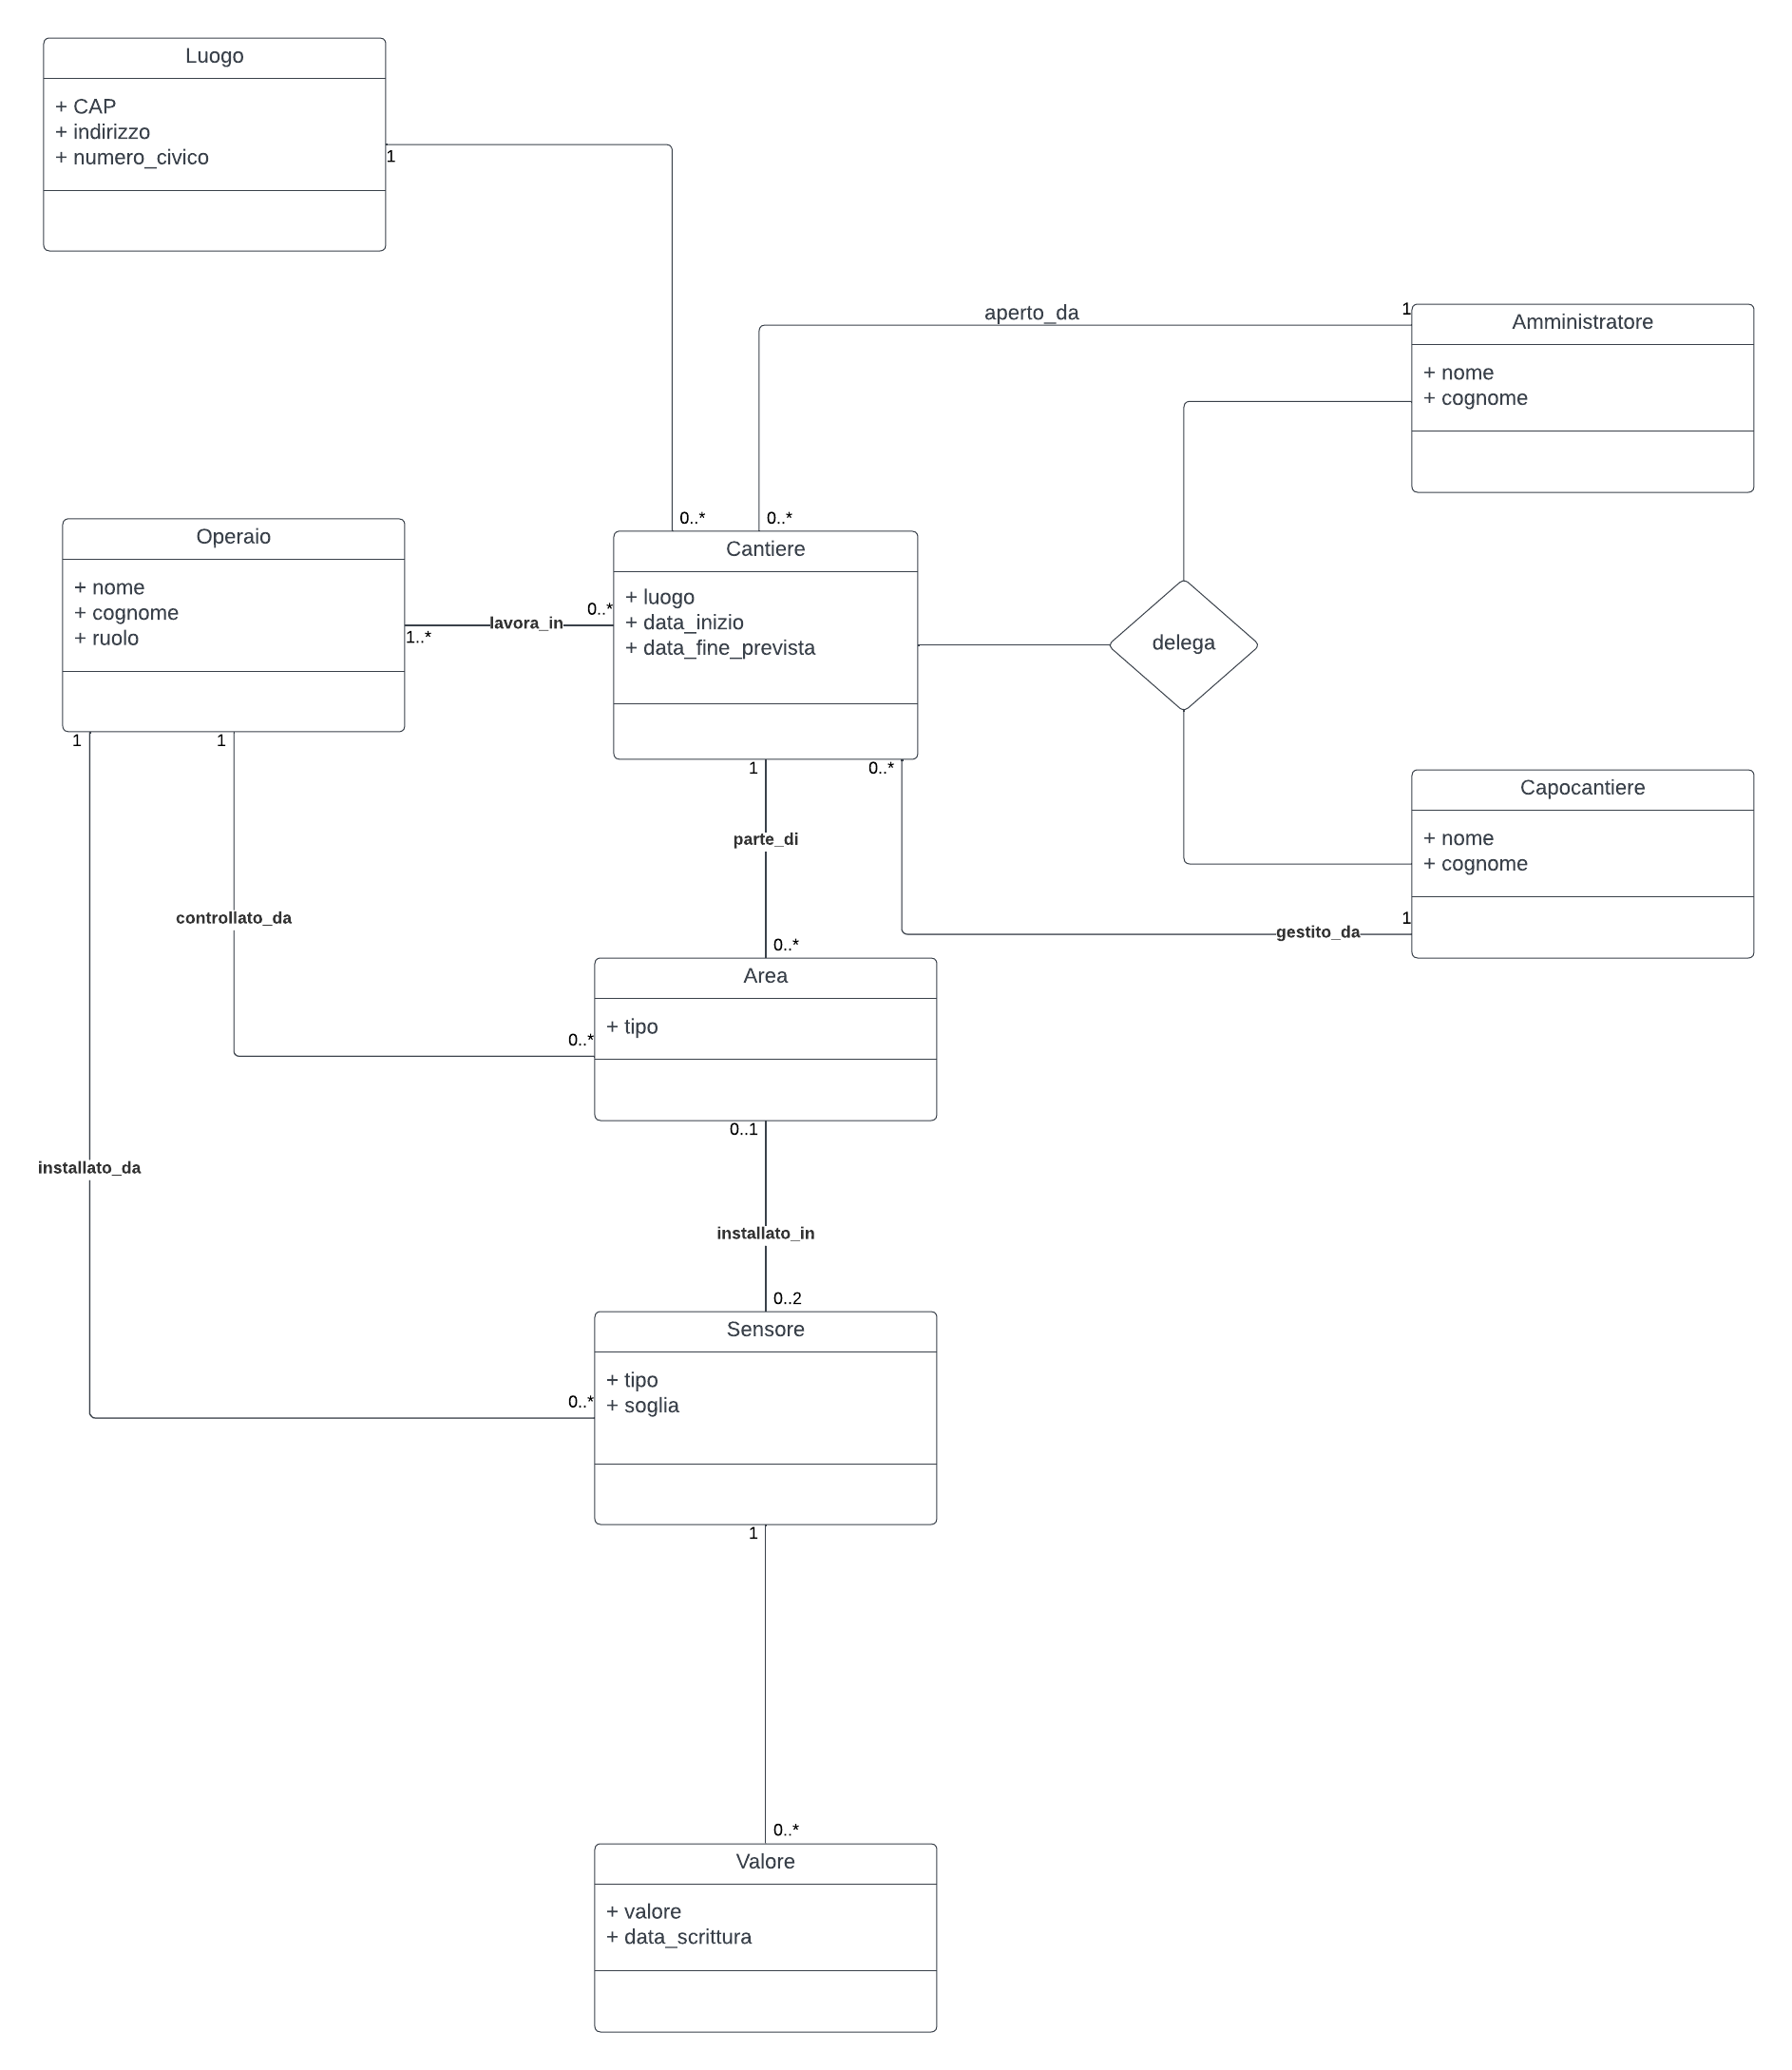
\includegraphics[scale=0.5]{cantiereconcettualeristr.png}\)
\section*{Progettazione Logica}
\label{sec:orgbb0f897}
\subsection*{Convenzione}
\label{sec:orgca9e6a2}
Nella prossima sezione verranno indicate con una singola sottolineatura le chiavi \(\underline{primarie}\), mentre le chiavi \(\underline{\underline{esterne}}\) con una doppia sottolineatura.
\subsection*{Traduzione}
\label{sec:org2c2636c}
\begin{itemize}
\item \textbf{Cantiere} (\textbf{\(\underline{id}\)}, data␣inizio, data␣fine␣prevista, \(\underline{\underline{id\textunderscore luogo}}\), \(\underline{\underline{aperto\textunderscore da}}\), \(\underline{\underline{gestito\textunderscore da}}\))
\begin{itemize}
\item \textbf{aperto da} \(\rightarrow\) Amministratore.\(id\)
\item \textbf{gestito da} \(\rightarrow\) Capocantiere.\(id\)
\item \textbf{\(id\textunderscore luogo\)} \(\rightarrow\) Luogo.\(id\)
\end{itemize}
\item \textbf{Area} (\textbf{\(\underline{id}\)}, tipo, \(\underline{\underline{parte\textunderscore di}}\), \(\underline{\underline{controllato\textunderscore da}}\))
\begin{itemize}
\item \textbf{parte di} \(\rightarrow\) Cantiere.\(id\)
\item \textbf{controllato da} \(\rightarrow\) Operaio.\(id\)
\end{itemize}
\item \textbf{Sensore} (\textbf{\(\underline{id}\)}, tipo, \(\underline{\underline{installato\textunderscore da}}\), \(\underline{\underline{installato\textunderscore in}}\))
\begin{itemize}
\item \textbf{installato da} \(\rightarrow\) Operaio.\(id\)
\item \textbf{installato in} \(\rightarrow\) Area.\(id\)
\end{itemize}
\item \textbf{Valore} (valore, \textbf{\(\underline{data_scrittura}\)}, \(\underline{\underline{valore\textunderscore di}}\))
\begin{itemize}
\item \textbf{valore di} \(\rightarrow\) Sensore.\(id\)
\end{itemize}
\item \textbf{Amministratore} (\textbf{\(\underline{id}\)}, nome, cognome)
\item \textbf{Capocantiere} (\textbf{\(\underline{id}\)}, nome, cognome)
\item \textbf{Operaio} (\textbf{\(\underline{id}\)}, nome, cognome, ruolo)
\item \textbf{Luogo} (\textbf{\(\underline{id}\)}, CAP, indirizzo, \(numero\textunderscore civico\))
\item \textbf{Delega} (\(\underline{\underline{cantiere\textunderscore id}}\), \(\underline{\underline{amministratore\textunderscore id}}\), \(\underline{\underline{capocantiere\textunderscore id}}\))
\begin{itemize}
\item \textbf{\(cantiere\textunderscore id\)} \(\rightarrow\) Cantiere.\(id\)
\item \textbf{\(amministratore\textunderscore id\)} \(\rightarrow\) Amministratore.\(id\)
\item \textbf{capocantiere\textunderscore id} \(\rightarrow\) Capocantiere.\(id\)
\end{itemize}
\item \textbf{Lavora in}  (\(\underline{\underline{operaio\textunderscore id}}\), \(\underline{\underline{cantiere\textunderscore id}}\))
\begin{itemize}
\item \textbf{\(cantiere\textunderscore id\)} \(\rightarrow\) Cantiere.\(id\)
\item \textbf{\(operaio\textunderscore id\)} \(\rightarrow\) Operaio.\(id\)
\end{itemize}
\end{itemize}
\section*{Progettazione Fisica}
\label{sec:org8d6a1aa}
\subsection*{Scelta del DBMS}
\label{sec:orga90631d}
La base dati é stata realizzata con il DBMS \href{https://www.postgresql.org/}{Postgres}.
Una peculiaritá di questo DBMS é che non implementa le \uline{ASSERTION}, queste sono state implementate tramite \uline{PROCEDURES} e \uline{TRIGGER}.
In particolare per implementare una assertion vi é una procedura che si occupa di effettuare il controllo del vincolo e un trigger il cui compito é chiamare la procedura.
Tutti i dettagli possono essere consultati nella sezione successiva dell'SQL.
\subsection*{Creazione Database}
\label{sec:org29b63f4}
\begin{verbatim}
CREATE DATABASE cantiere
    WITH
    OWNER = postgres
    ENCODING = 'UTF8'
    LC_COLLATE = 'en_US.utf8'
    LC_CTYPE = 'en_US.utf8'
    TABLESPACE = pg_default
    CONNECTION LIMIT = -1
    IS_TEMPLATE = False;
\end{verbatim}
\subsection*{Creazione dello schema}
\label{sec:org8fc7f62}
\begin{verbatim}
CREATE SCHEMA IF NOT EXISTS cantiere
    AUTHORIZATION postgres;
\end{verbatim}
\subsection*{Definizione enumerazioni}
\label{sec:org9c1326a}
\begin{itemize}
\item Enumerazione ruolo
\label{sec:org71a97f5}
\begin{verbatim}
CREATE TYPE cantiere.ruolo AS ENUM
    ('semplice', 'idraulico', 'macchinista', 'elettricista', 'operatore');
\end{verbatim}
\item Enumerazione zona
\label{sec:org00396a0}
\begin{verbatim}
CREATE TYPE cantiere.zona AS ENUM
    ('servizi_pubblici', 'zona_verde', 'zona_residenziale', 'zona_ristorazione');
\end{verbatim}
\item Enumerazione tipo
\label{sec:orgae25546}
\begin{verbatim}
CREATE TYPE cantiere.tipo AS ENUM
       ('gas', 'rumore');
\end{verbatim}
\end{itemize}
\subsection*{Definizione tabelle}
\label{sec:org4d2f052}
\begin{itemize}
\item Tabella amministratore
\label{sec:orgc811e33}
\begin{verbatim}
CREATE TABLE cantiere.amministratore(
       id SERIAL PRIMARY KEY,
       nome VARCHAR(50) NOT NULL,
       cognome VARCHAR(50) NOT NULL);
\end{verbatim}
\item Tabella capocantiere
\label{sec:org41da6fd}
\begin{verbatim}
CREATE TABLE cantiere.capocantiere(
       id SERIAL PRIMARY KEY,
       nome VARCHAR(50) NOT NULL,
       cognome VARCHAR(50) NOT NULL);
\end{verbatim}
\item Tabella luogo
\label{sec:orgd893d71}
\begin{verbatim}
CREATE TABLE cantiere.luogo(
       id SERIAL PRIMARY KEY,
       citta VARCHAR(50) NOT NULL,
       CAP VARCHAR(5) NOT NULL,
       indirizzo VARCHAR(50) NOT NULL,
       numero_civico INT);
\end{verbatim}
\item Tabella cantiere
\label{sec:org9c8abad}
\begin{verbatim}
CREATE TABLE cantiere.cantiere(
       id SERIAL PRIMARY KEY,
       data_inizio DATE NOT NULL,
       data_fine_prevista DATE NOT NULL,
       aperto_da SERIAL,
       luogo_id SERIAL,
       FOREIGN KEY (luogo_id)
               REFERENCES
                cantiere.luogo(id)
                    ON UPDATE CASCADE,
       FOREIGN KEY (aperto_da)
               REFERENCES
                cantiere.amministratore(id)
                    ON UPDATE CASCADE);
\end{verbatim}
\item Tabella operaio
\label{sec:org73dda9f}
\begin{verbatim}
CREATE TABLE cantiere.operaio(
       id SERIAL PRIMARY KEY,
       nome VARCHAR(50) NOT NULL,
       cognome VARCHAR(50) NOT NULL,
       ruolo cantiere.RUOLO);

ALTER TABLE cantiere.operaio
            ALTER COLUMN ruolo SET DEFAULT 'semplice';
\end{verbatim}
\item Tabella area
\label{sec:orgdb3decd}
\begin{verbatim}
CREATE TABLE cantiere.area(
       id SERIAL PRIMARY KEY,
       zona cantiere.ZONA NOT NULL,
       parte_di SERIAL,
       controllato_da SERIAL,
       FOREIGN KEY(parte_di)
               REFERENCES cantiere.cantiere(id)
                          ON DELETE CASCADE
                          ON UPDATE CASCADE,
       FOREIGN KEY(controllato_da)
               REFERENCES cantiere.operaio(id)
                          ON UPDATE CASCADE);
\end{verbatim}
\item Tabella sensore
\label{sec:org12625cf}
\begin{verbatim}
CREATE TABLE cantiere.sensore(
       id SERIAL PRIMARY KEY,
       tipo cantiere.TIPO NOT NULL,
       soglia FLOAT8 NOT NULL,
       installato_da SERIAL,
       installato_in SERIAL,
       FOREIGN KEY(installato_da)
               REFERENCES cantiere.operaio(id)
                          ON UPDATE CASCADE
                          ON DELETE SET NULL,
       FOREIGN KEY(installato_in)
               REFERENCES cantiere.area(id)
                          ON UPDATE CASCADE
                          ON DELETE CASCADE);
\end{verbatim}
\item Tabella valore
\label{sec:orgdd210f2}
\begin{verbatim}
CREATE TABLE cantiere.valore(
       data_scrittura TIMESTAMP,
       valore_di SERIAL,
       valore FLOAT8 NOT NULL,
       PRIMARY KEY(data_scrittura, valore_di),
       FOREIGN KEY(valore_di)
               REFERENCES cantiere.sensore(id)
                          ON UPDATE CASCADE
                          ON DELETE CASCADE);
\end{verbatim}
\item Tabella lavora\textsubscript{in}
\label{sec:org96f7bd3}
\begin{verbatim}
CREATE TABLE cantiere.lavora_in(
       cantiere_id SERIAL,
       operaio_id SERIAL,
       PRIMARY KEY(cantiere_id, operaio_id),
       FOREIGN KEY(cantiere_id)
               REFERENCES cantiere.cantiere(id)
                          ON UPDATE CASCADE
                          ON DELETE CASCADE,
       FOREIGN KEY(operaio_id)
               REFERENCES cantiere.operaio(id)
                          ON UPDATE CASCADE
                          ON DELETE CASCADE);
\end{verbatim}
\item Tabella delega
\label{sec:org1a3d53d}
\begin{verbatim}
CREATE TABLE cantiere.delega(
       cantiere_id SERIAL,
       amministratore_id SERIAL,
       capocantiere_id SERIAL,
       PRIMARY KEY(cantiere_id, amministratore_id, capocantiere_id),
       FOREIGN KEY(cantiere_id)
               REFERENCES cantiere.cantiere(id)
                          ON DELETE CASCADE
                          ON UPDATE CASCADE,
       FOREIGN KEY(capocantiere_id)
               REFERENCES cantiere.capocantiere(id)
                          ON DELETE CASCADE
                          ON UPDATE CASCADE,
       FOREIGN KEY(amministratore_id)
               REFERENCES cantiere.amministratore(id)
                          ON DELETE CASCADE
                          ON UPDATE CASCADE);
\end{verbatim}
\end{itemize}
\subsection*{Definizione vincoli}
\label{sec:orge158d43}
Postgres non possiede un meccanismo ad-hoc per definire dei vincoli, lo stesso comportamento puó essere ottenuto tramite una procedura ed un trigger.
\begin{itemize}
\item Vincolo delega univoca
\label{sec:org7700261}
\begin{verbatim}
CREATE OR REPLACE FUNCTION
cantiere.delega_univoca()
RETURNS TRIGGER
LANGUAGE plpgsql
AS $$
DECLARE
BEGIN
    IF EXISTS(SELECT *
              FROM cantiere.delega AS d
              WHERE d.cantiere_id = NEW.cantiere_id
                    AND d.amministratore_id = NEW.amministratore_id)
    THEN
        RAISE EXCEPTION 'il cantiere [%] é stato gía delegato', NEW.cantiere_id;
    ELSE
        RETURN NEW;
    END IF;
END;
$$

CREATE OR REPLACE TRIGGER delega_univoca_trig
BEFORE INSERT OR UPDATE ON cantiere.delega
FOR EACH ROW
    EXECUTE PROCEDURE cantiere.delega_univoca();
\end{verbatim}
\item Vincolo valore non supera soglia
\label{sec:orgc2ef7f4}
\begin{verbatim}
CREATE OR REPLACE FUNCTION
cantiere.valore_non_supera_soglia()
RETURNS TRIGGER
LANGUAGE plpgsql
AS $$
DECLARE
    soglia FLOAT8 := 0;
BEGIN
    SELECT s.soglia INTO soglia
    FROM cantiere.sensore AS s
    WHERE s.id = NEW.valore_di;

    IF soglia < NEW.valore
    THEN
        RAISE EXCEPTION '[Allarme] il sensore % ha superato la soglia: %', NEW.valore_di, soglia;
    ELSE
        RETURN NEW;
    END IF;
END;
$$

CREATE OR REPLACE TRIGGER valore_non_supera_soglia_trig
BEFORE INSERT OR UPDATE ON cantiere.valore
FOR EACH ROW
    EXECUTE PROCEDURE cantiere.valore_non_supera_soglia();
\end{verbatim}
\item Vincolo data fine plausibile
\label{sec:orga66bf08}
\begin{verbatim}
CREATE OR REPLACE FUNCTION
cantiere.data_fine_plausibile()
RETURNS TRIGGER
LANGUAGE plpgsql
AS $$
DECLARE
BEGIN
    IF NEW.data_inizio >= NEW.data_fine_prevista
    THEN
        RAISE EXCEPTION 'la data di fine lavori é antecedente a quella di inizio';
    ELSE
        RETURN NEW;
    END IF;
END;
$$

CREATE OR REPLACE TRIGGER data_fine_plausibile_trig
BEFORE INSERT OR UPDATE ON cantiere.cantiere
FOR EACH ROW
    EXECUTE PROCEDURE cantiere.data_fine_plausibile();
\end{verbatim}
\item Vincolo data nuova scrittura
\label{sec:org3154e23}
\begin{verbatim}
CREATE OR REPLACE FUNCTION
cantiere.data_nuova_scrittura()
RETURNS TRIGGER
LANGUAGE plpgsql
AS $$
DECLARE
    ultima_scrittura DATE := NULL;
BEGIN
    SELECT v.data_scrittura INTO ultima_scrittura
    FROM cantiere.valore AS v
    WHERE v.valore_di = NEW.valore_di
    ORDER BY v.data_scrittura DESC
    LIMIT 1;

    IF ultima_scrittura >= NEW.data_scrittura
    THEN
        RAISE EXCEPTION 'impossibile inserire una scrittura meno recente';
    ELSE
        RETURN NEW;
    END IF;
END;
$$

CREATE OR REPLACE TRIGGER data_nuova_scrittura_trig
BEFORE INSERT OR UPDATE ON cantiere.valore
FOR EACH ROW
    EXECUTE PROCEDURE cantiere.data_nuova_scrittura();
\end{verbatim}
\item Vincolo amministratore delega
\label{sec:orgc748f8e}
\begin{verbatim}
CREATE OR REPLACE FUNCTION
cantiere.amministratore_corretto_delega()
RETURNS TRIGGER
LANGUAGE plpgsql
AS $$
DECLARE
    amministratore_id INTEGER;
BEGIN
    SELECT c.aperto_da INTO amministratore_id
    FROM cantiere.cantiere AS c
    WHERE c.id = NEW.cantiere_id;
    IF amministratore_id <> NEW.amministratore_id
    THEN
        RAISE EXCEPTION 'il cantiere é stato aperto da un altro amministratore';
    ELSE
        RETURN NEW;
    END IF;
END;
$$

CREATE OR REPLACE TRIGGER amministratore_corretto_delega_trig
BEFORE INSERT OR UPDATE ON cantiere.delega
FOR EACH ROW
    EXECUTE PROCEDURE cantiere.amministratore_corretto_delega();
\end{verbatim}
\item Vincolo solo operatore installa sensore
\label{sec:org5d9d1fb}
\begin{verbatim}
CREATE OR REPLACE FUNCTION
cantiere.solo_operatore_installa_sensore()
RETURNS TRIGGER
LANGUAGE plpgsql
AS $$
DECLARE
    ruolo cantiere.RUOLO;
BEGIN
    SELECT o.ruolo INTO ruolo
    FROM cantiere.operaio AS o
    WHERE o.id = NEW.installato_da;
    IF ruolo <> 'operatore'
    THEN
        RAISE EXCEPTION '% non é un operatore', NEW.installato_da;
    ELSE
        RETURN NEW;
    END IF;
END;
$$

CREATE OR REPLACE TRIGGER solo_operatore_installa_sensore_trig
BEFORE INSERT OR UPDATE ON cantiere.sensore
FOR EACH ROW
    EXECUTE PROCEDURE cantiere.solo_operatore_installa_sensore();
\end{verbatim}
\item Vincolo numero civico naturale
\label{sec:orge60f458}
\begin{verbatim}
CREATE OR REPLACE FUNCTION
cantiere.numero_civico_naturale()
RETURNS TRIGGER
LANGUAGE plpgsql
AS $$
DECLARE
BEGIN
    IF NEW.numero_civico <= 0
    THEN
        RAISE EXCEPTION 'Il numero civico deve essere positivo';
    ELSE
        RETURN NEW;
    END IF;
END;
$$

CREATE OR REPLACE TRIGGER solo_operatore_installa_sensore_trig
BEFORE INSERT OR UPDATE ON cantiere.luogo
FOR EACH ROW
    EXECUTE PROCEDURE cantiere.numero_civico_naturale();
\end{verbatim}
\item Vincolo max due sensori differenti
\label{sec:orge6a1483}
\begin{verbatim}
CREATE OR REPLACE FUNCTION
cantiere.max_due_sensori_differenti()
RETURNS TRIGGER
LANGUAGE plpgsql
AS $$
DECLARE
    already_installed RECORD := NULL;
BEGIN
    SELECT * INTO already_installed
    FROM cantiere.sensore AS s
    WHERE s.installato_in = NEW.installato_in AND s.tipo = NEW.tipo;
    IF already_installed <> NULL
    THEN
        RAISE EXCEPTION 'sensore di tipo % giá installato in %', NEW.tipo, NEW.installato_in;
    ELSE
        RETURN NEW;
    END IF;
END;
$$

CREATE OR REPLACE TRIGGER max_due_sensori_differenti_trig
BEFORE INSERT OR UPDATE ON cantiere.sensore
FOR EACH ROW
    EXECUTE PROCEDURE cantiere.max_due_sensori_differenti();
\end{verbatim}
\item Vincolo CAP\textsubscript{ha}\textsubscript{5}\textsubscript{caratteri}
\label{sec:org9e76fd9}
\begin{verbatim}
CREATE OR REPLACE FUNCTION
cantiere.CAP_ha_5_caratteri()
RETURNS TRIGGER
LANGUAGE plpgsql
AS $$
DECLARE
BEGIN
    IF LENGTH(NEW.CAP) <> 5
    THEN
        RAISE EXCEPTION 'Il CAP deve essere composto di 5 cifre, [%] non é valido', NEW.CAP;
    ELSE
        RETURN NEW;
    END IF;
END;
$$

CREATE OR REPLACE TRIGGER CAP_ha_5_caratteri_trig
BEFORE INSERT OR UPDATE ON cantiere.luogo
FOR EACH ROW
    EXECUTE PROCEDURE cantiere.CAP_ha_5_caratteri();
\end{verbatim}
\item Vincolo CAP composto solo da cifre
\label{sec:org2b31737}
\begin{verbatim}
CREATE OR REPLACE FUNCTION
cantiere.CAP_composto_solo_da_cifre()
RETURNS TRIGGER
LANGUAGE plpgsql
AS $$
DECLARE
BEGIN
    IF LENGTH(REGEXP_REPLACE(NEW.CAP, '[^0-9]', '', 'g')) <> 5
    THEN
        RAISE EXCEPTION '[%] CAP non valido, contiene valori non numerici', NEW.CAP;
    ELSE
        RETURN NEW;
    END IF;
END;
$$

CREATE OR REPLACE TRIGGER CAP_composto_solo_da_cifre_trig
BEFORE INSERT OR UPDATE ON cantiere.luogo
FOR EACH ROW
    EXECUTE PROCEDURE cantiere.CAP_composto_solo_da_cifre();
\end{verbatim}
\item Vincolo luogo univoco
\label{sec:orgd0a2622}
\begin{verbatim}
CREATE OR REPLACE FUNCTION
cantiere.luogo_univoco()
RETURNS TRIGGER
LANGUAGE plpgsql
AS $$
DECLARE
    luogo RECORD := NULL;
BEGIN
    SELECT * INTO luogo
    FROM cantiere.luogo AS l
    WHERE l.CAP = NEW.CAP AND
          l.indirizzo = NEW.indirizzo AND
          l.numero_civico = NEW.numero_civico AND
          l.citta = new.citta;

    IF luogo <> NULL
    THEN
        RAISE EXCEPTION 'Luogo giá presente';
    ELSE
        RETURN NEW;
    END IF;
END;
$$

CREATE OR REPLACE TRIGGER luogo_univoco_trig
BEFORE INSERT OR UPDATE ON cantiere.luogo
FOR EACH ROW
    EXECUTE PROCEDURE cantiere.luogo_univoco();
\end{verbatim}
\item Vincolo area univoca cantiere
\label{sec:orgcf7bc4b}
\begin{verbatim}
CREATE OR REPLACE FUNCTION
cantiere.area_univoca_per_cantiere()
RETURNS TRIGGER
LANGUAGE plpgsql
AS $$
DECLARE
    area RECORD := NULL;
BEGIN
    SELECT * INTO area
    FROM cantiere.area AS a
    WHERE a.tipo = NEW.tipo;
    IF area <> NULL
    THEN
        RAISE EXCEPTION 'Area giá presente nel cantiere';
    ELSE
        RETURN NEW;
    END IF;
END;
$$

CREATE OR REPLACE TRIGGER area_univoca_per_cantiere_trig
BEFORE INSERT OR UPDATE ON cantiere.area
FOR EACH ROW
    EXECUTE PROCEDURE cantiere.area_univoca_per_cantiere();
\end{verbatim}
\item Vincolo valore scritto positivo
\label{sec:org187217a}
\begin{verbatim}
CREATE OR REPLACE FUNCTION
cantiere.valore_scritto_positivo()
RETURNS TRIGGER
LANGUAGE plpgsql
AS $$
DECLARE
BEGIN
    IF NEW.valore < 0
    THEN
        RAISE EXCEPTION 'Il valore da associare ad una scrittura deve essere positivo';
    ELSE
        RETURN NEW;
    END IF;
END;
$$

CREATE OR REPLACE TRIGGER valore_scritto_positivo_trig
BEFORE INSERT OR UPDATE ON cantiere.valore
FOR EACH ROW
    EXECUTE PROCEDURE cantiere.valore_scritto_positivo();
\end{verbatim}
\item Vincolo data scrittura dopo inizio lavori
\label{sec:org9661cae}
\begin{verbatim}
CREATE OR REPLACE FUNCTION
cantiere.data_scrittura_dopo_inizio_lavori()
RETURNS TRIGGER
LANGUAGE plpgsql
AS $$
DECLARE
    sensore RECORD := NULL;
    inizio_lavori TIMESTAMP := NULL;
BEGIN
    SELECT c.data_inizio::timestamp INTO inizio_lavori
    FROM cantiere.cantiere AS C
    WHERE c.id = (SELECT a.parte_di
                  FROM cantiere.area AS a
                  WHERE  a.id = (
                         SELECT s.installato_in
                         FROM cantiere.sensore AS s
                         WHERE s.id = NEW.valore_di));
    
    IF NEW.data_scrittura <= inizio_lavori
    THEN
        RAISE EXCEPTION 'La lettura é antecedente ai lavori.';
    ELSE
        RETURN NEW;
    END IF;
END;
$$

CREATE OR REPLACE TRIGGER valore_scritto_positivo_trig
BEFORE INSERT OR UPDATE ON cantiere.valore
FOR EACH ROW
    EXECUTE PROCEDURE cantiere.data_scrittura_dopo_inizio_lavori();
\end{verbatim}
\end{itemize}
\section*{Popolazione della base dati}
\label{sec:org12a2614}
\subsection*{Operaio}
\label{sec:org1bdac36}
\begin{verbatim}
INSERT INTO cantiere.operaio(nome, cognome, ruolo) VALUES
('Mario', 'Rossi', 'semplice'),
('Pasquale', 'Esposito', 'idraulico'),
('Ciro', 'Esposito', 'macchinista'),
('Jose', 'Miranda', 'elettricista'),
('Chief', 'Braga', 'operatore'),

('Mario', 'Verdi', 'semplice'),
('René', 'Ferretti', 'idraulico'),
('Giuseppe', 'Verdi', 'macchinista'),
('Valerio', 'Brida', 'elettricista'),
('Michele', 'Sua', 'operatore'),

('Sergio', 'Lang', 'semplice'),
('Alessandro', 'Roma', 'idraulico'),
('Domenico', 'Bini', 'macchinista'),
('Mirco', 'Sorrentino', 'elettricista'),
('Antonio', 'Petrillo', 'operatore'),

('Gerardo', 'Pujaz', 'semplice'),
('Bernardo', 'Lico', 'idraulico'),
('Christian', 'Ice', 'macchinista'),
('Matteo', 'Montesi', 'elettricista'),
('Gerardo', 'Malanga', 'operatore');
\end{verbatim}
\subsection*{Capocantiere}
\label{sec:org9ab004d}
\begin{verbatim}
INSERT INTO cantiere.capocantiere(nome, cognome) VALUES
('Francesco', 'Petrillo'),
('Domenico', 'Petrillo'),
('Manuel', 'Scarpitta');
\end{verbatim}
\subsection*{Amministratore}
\label{sec:orgc869211}
\begin{verbatim}
INSERT INTO cantiere.amministratore(nome, cognome) VALUES
('Mr', 'Implenia'),
('Richard', 'Benson');
\end{verbatim}
\subsection*{Luogo}
\label{sec:org44bb169}
\begin{verbatim}
INSERT INTO cantiere.luogo(citta, cap, indirizzo, numero_civico) VALUES
('San Giovanni a Piro','84070', 'Via Iacine', 3),
('Fuorigrotta', '80125', 'Via Mercantini', 10),
('Montreaux', '19200', 'Rue du Guercet', 5);
\end{verbatim}
\subsection*{Cantiere}
\label{sec:org742fa40}
\begin{verbatim}
INSERT INTO cantiere.cantiere(data_inizio, data_fine_prevista, luogo_id, aperto_da) VALUES
('2019-07-17', '2019-08-16', 4, 1),
('2000-02-09', '2005-06-1', 2, 2),
('2023-07-1', '2023-08-30', 3, 1);
\end{verbatim}
\subsection*{Area}
\label{sec:orgd696960}
\begin{verbatim}
INSERT INTO cantiere.area(zona, parte_di, controllato_da) VALUES
('servizi_pubblici', 5, 15),
('zona_verde', 5, 15),
('zona_residenziale', 5, 18),
('zona_ristorazione', 5, 18),
('servizi_pubblici', 4, 13),
('zona_verde', 4, 20),
('servizi_pubblici', 6, 7),
('zona_ristorazione', 6, 5),
('zona_verde', 6, 11);
\end{verbatim}
\subsection*{Sensore}
\label{sec:orgf4bed6d}
\begin{verbatim}
INSERT INTO cantiere.sensore(tipo, installato_da, installato_in, soglia) VALUES
('gas', 15, 1, 200),
('rumore', 15, 1, 300),
('gas', 15, 2, 200),
('rumore', 15, 2, 300),
('gas', 15, 3, 200),
('rumore', 15, 3, 300),
('gas', 15, 4, 200),
('rumore', 15, 4, 300),
('gas', 5, 5, 400),
('gas', 10, 6, 300),
('rumore', 10, 6, 100),
('rumore', 20, 7, 800),
('gas', 20, 8, 250),
('rumore', 20, 9, 100);
\end{verbatim}
\subsection*{Valore}
\label{sec:org2904ba6}
\subsubsection*{Sensore 1}
\label{sec:orgb555013}
\begin{verbatim}
INSERT INTO cantiere.valore(data_scrittura, valore_di, valore) VALUES
('2000-05-12 00:00:00-07', 1, 150),
('2000-05-12 01:00:00-07', 1, 50),
('2001-05-12 02:00:00-07', 1, 75),
('2001-05-12 03:00:00-07', 1, 95),
('2002-05-12 04:00:00-07', 1, 100),
('2002-05-12 05:00:00-07', 1, 50),
('2003-05-12 06:00:00-07', 1, 28),
('2003-05-12 07:00:00-07', 1, 50),
('2004-05-12 08:00:00-07', 1, 60);
\end{verbatim}
\subsubsection*{Sensore 2}
\label{sec:org6199ade}
\begin{verbatim}
INSERT INTO cantiere.valore(data_scrittura, valore_di, valore) VALUES
('2000-05-12 00:00:00-07', 2, 150),
('2000-05-12 01:00:00-07', 2, 50),
('2001-05-12 02:00:00-07', 2, 75),
('2001-05-12 03:00:00-07', 2, 95),
('2002-05-12 04:00:00-07', 2, 100),
('2002-05-12 05:00:00-07', 2, 50),
('2003-05-12 06:00:00-07', 2, 28),
('2003-05-12 07:00:00-07', 2, 50),
('2004-05-12 08:00:00-07', 2, 60);
\end{verbatim}
\subsubsection*{Sensore 3}
\label{sec:orgf3a34b3}
\begin{verbatim}
INSERT INTO cantiere.valore(data_scrittura, valore_di, valore) VALUES
('2000-05-12 00:00:00-07', 3, 150),
('2000-05-12 01:00:00-07', 3, 50),
('2001-05-12 02:00:00-07', 3, 75),
('2001-05-12 03:00:00-07', 3, 95),
('2002-05-12 04:00:00-07', 3, 100),
('2002-05-12 05:00:00-07', 3, 50),
('2003-05-12 06:00:00-07', 3, 28),
('2003-05-12 07:00:00-07', 3, 50),
('2004-05-12 08:00:00-07', 3, 60);
\end{verbatim}
\subsubsection*{Sensore 4}
\label{sec:org9d92b6f}
\begin{verbatim}
INSERT INTO cantiere.valore(data_scrittura, valore_di, valore) VALUES
('2000-05-12 00:00:00-07', 4, 150),
('2000-05-12 01:00:00-07', 4, 50),
('2001-05-12 02:00:00-07', 4, 75),
('2001-05-12 03:00:00-07', 4, 95),
('2002-05-12 04:00:00-07', 4, 100),
('2002-05-12 05:00:00-07', 4, 50),
('2003-05-12 06:00:00-07', 4, 28),
('2003-05-12 07:00:00-07', 4, 50),
('2004-05-12 08:00:00-07', 4, 60);
\end{verbatim}
\subsubsection*{Sensore 5}
\label{sec:org739c6dc}
\begin{verbatim}
INSERT INTO cantiere.valore(data_scrittura, valore_di, valore) VALUES
('2000-05-12 00:00:00-07', 5, 150),
('2000-05-12 01:00:00-07', 5, 50),
('2001-05-12 02:00:00-07', 5, 75),
('2001-05-12 03:00:00-07', 5, 95),
('2002-05-12 04:00:00-07', 5, 100),
('2002-05-12 05:00:00-07', 5, 50),
('2003-05-12 06:00:00-07', 5, 28),
('2003-05-12 07:00:00-07', 5, 50),
('2004-05-12 08:00:00-07', 5, 60);
\end{verbatim}
\subsubsection*{Sensore 6}
\label{sec:org5362042}
\begin{verbatim}
INSERT INTO cantiere.valore(data_scrittura, valore_di, valore) VALUES
('2000-05-12 00:00:00-07', 6, 150),
('2000-05-12 01:00:00-07', 6, 50),
('2001-05-12 02:00:00-07', 6, 75),
('2001-05-12 03:00:00-07', 6, 95),
('2002-05-12 04:00:00-07', 6, 100),
('2002-05-12 05:00:00-07', 6, 50),
('2003-05-12 06:00:00-07', 6, 28),
('2003-05-12 07:00:00-07', 6, 50),
('2004-05-12 08:00:00-07', 6, 60);
\end{verbatim}
\subsubsection*{Sensore 7}
\label{sec:org7763171}
\begin{verbatim}
INSERT INTO cantiere.valore(data_scrittura, valore_di, valore) VALUES
('2000-05-12 00:00:00-07', 7, 150),
('2000-05-12 01:00:00-07', 7, 50),
('2001-05-12 02:00:00-07', 7, 75);
\end{verbatim}
\subsubsection*{Sensore 8}
\label{sec:orgb2e50b6}
\begin{verbatim}
INSERT INTO cantiere.valore(data_scrittura, valore_di, valore) VALUES
('2000-05-12 00:00:00-07', 8, 150),
('2000-05-12 01:00:00-07', 8, 50),
('2001-05-12 02:00:00-07', 8, 75);
\end{verbatim}
\subsubsection*{Sensore 9}
\label{sec:org691788f}
\begin{verbatim}
INSERT INTO cantiere.valore(data_scrittura, valore_di, valore) VALUES
('2000-05-12 00:00:00-07', 9, 150),
('2000-05-12 01:00:00-07', 9, 50),
('2001-05-12 02:00:00-07', 9, 75);
\end{verbatim}
\subsubsection*{Sensore 10}
\label{sec:orgabb3682}
\begin{verbatim}
INSERT INTO cantiere.valore(data_scrittura, valore_di, valore) VALUES
('2000-05-12 00:00:00-07', 10, 150),
('2000-05-12 01:00:00-07', 10, 50),
('2001-05-12 02:00:00-07', 10, 75);
\end{verbatim}
\subsubsection*{Sensore 11}
\label{sec:org7dd0c97}
\begin{verbatim}
INSERT INTO cantiere.valore(data_scrittura, valore_di, valore) VALUES
('2000-05-12 00:00:00-07', 11, 150),
('2000-05-12 01:00:00-07', 11, 50),
('2001-05-12 02:00:00-07', 11, 75);
\end{verbatim}
\subsubsection*{Sensore 12}
\label{sec:orgbef0b4d}
\begin{verbatim}
INSERT INTO cantiere.valore(data_scrittura, valore_di, valore) VALUES
('2000-05-12 00:00:00-07', 12, 150),
('2000-05-12 01:00:00-07', 12, 50),
('2001-05-12 02:00:00-07', 12, 75);
\end{verbatim}
\subsubsection*{Sensore 13}
\label{sec:org7de6ab3}
\begin{verbatim}
INSERT INTO cantiere.valore(data_scrittura, valore_di, valore) VALUES
('2000-05-12 00:00:00-07', 13, 150),
('2000-05-12 01:00:00-07', 13, 50),
('2001-05-12 02:00:00-07', 13, 75);
\end{verbatim}
\subsubsection*{Sensore 14}
\label{sec:org53e5744}
\begin{verbatim}
INSERT INTO cantiere.valore(data_scrittura, valore_di, valore) VALUES
('2000-05-12 00:00:00-07', 14, 150),
('2000-05-12 01:00:00-07', 14, 50),
('2001-05-12 02:00:00-07', 14, 75);
\end{verbatim}
\subsubsection*{Sensore 15}
\label{sec:orgedd513e}
\begin{verbatim}
INSERT INTO cantiere.valore(data_scrittura, valore_di, valore) VALUES
('2000-05-12 00:00:00-07', 15, 150),
('2000-05-12 01:00:00-07', 15, 50),
('2001-05-12 02:00:00-07', 15, 75);
\end{verbatim}
\subsubsection*{Sensore 16}
\label{sec:org848921a}
\begin{verbatim}
INSERT INTO cantiere.valore(data_scrittura, valore_di, valore) VALUES
('2000-05-12 00:00:00-07', 16, 150),
('2000-05-12 01:00:00-07', 16, 50),
('2001-05-12 02:00:00-07', 16, 75);
\end{verbatim}
\subsubsection*{Sensore 17}
\label{sec:org9fc0628}
\begin{verbatim}
INSERT INTO cantiere.valore(data_scrittura, valore_di, valore) VALUES
('2000-05-12 00:00:00-07', 17, 150),
('2000-05-12 01:00:00-07', 17, 50),
('2001-05-12 02:00:00-07', 17, 75);
\end{verbatim}
\subsubsection*{Sensore 18}
\label{sec:org4b1cdf2}
\begin{verbatim}
INSERT INTO cantiere.valore(data_scrittura, valore_di, valore) VALUES
('2000-05-12 00:00:00-07', 18, 150),
('2000-05-12 01:00:00-07', 18, 50),
('2001-05-12 02:00:00-07', 18, 75);
\end{verbatim}
\subsubsection*{Sensore 19}
\label{sec:org4f06596}
\begin{verbatim}
INSERT INTO cantiere.valore(data_scrittura, valore_di, valore) VALUES
('2000-05-12 00:00:00-07', 19, 150),
('2000-05-12 01:00:00-07', 19, 50),
('2001-05-12 02:00:00-07', 19, 75);
\end{verbatim}
\subsubsection*{Sensore 20}
\label{sec:org6182de0}
\begin{verbatim}
INSERT INTO cantiere.valore(data_scrittura, valore_di, valore) VALUES
('2000-05-12 00:00:00-07', 20, 150),
('2000-05-12 01:00:00-07', 20, 50),
('2001-05-12 02:00:00-07', 20, 75);
\end{verbatim}
\subsubsection*{Sensore 21}
\label{sec:org0347587}
\begin{verbatim}
INSERT INTO cantiere.valore(data_scrittura, valore_di, valore) VALUES
('2000-05-12 00:00:00-07', 21, 150),
('2000-05-12 01:00:00-07', 21, 50),
('2001-05-12 02:00:00-07', 21, 75);
\end{verbatim}
\subsubsection*{Sensore 22}
\label{sec:orge43d025}
\begin{verbatim}
INSERT INTO cantiere.valore(data_scrittura, valore_di, valore) VALUES
('2000-05-12 00:00:00-07', 22, 150),
('2000-05-12 01:00:00-07', 22, 50),
('2001-05-12 02:00:00-07', 22, 75);
\end{verbatim}
\subsubsection*{Sensore 23}
\label{sec:org1ca2d40}
\begin{verbatim}
INSERT INTO cantiere.valore(data_scrittura, valore_di, valore) VALUES
('2000-05-12 00:00:00-07', 23, 150),
('2000-05-12 01:00:00-07', 23, 50),
('2001-05-12 02:00:00-07', 23, 75);
\end{verbatim}
\subsubsection*{Sensore 24}
\label{sec:org2f79419}
\begin{verbatim}
INSERT INTO cantiere.valore(data_scrittura, valore_di, valore) VALUES
('2000-05-12 00:00:00-07', 24, 150),
('2000-05-12 01:00:00-07', 24, 50),
('2001-05-12 02:00:00-07', 24, 75);
\end{verbatim}
\subsubsection*{Sensore 25}
\label{sec:orgebd5748}
\begin{verbatim}
INSERT INTO cantiere.valore(data_scrittura, valore_di, valore) VALUES
('2000-05-12 00:00:00-07', 25, 100),
('2000-05-12 01:00:00-07', 25, 50),
('2001-05-12 02:00:00-07', 25, 75);
\end{verbatim}
\subsubsection*{Sensore 26}
\label{sec:org6138103}
\begin{verbatim}
INSERT INTO cantiere.valore(data_scrittura, valore_di, valore) VALUES
('2000-05-12 00:00:00-07', 26, 100),
('2000-05-12 01:00:00-07', 26, 50),
('2001-05-12 02:00:00-07', 26, 75);
\end{verbatim}
\subsubsection*{Sensore 27}
\label{sec:org7122576}
\begin{verbatim}
INSERT INTO cantiere.valore(data_scrittura, valore_di, valore) VALUES
('2000-05-12 00:00:00-07', 27, 100),
('2000-05-12 01:00:00-07', 27, 50),
('2001-05-12 02:00:00-07', 27, 75);
\end{verbatim}
\subsubsection*{Sensore 28}
\label{sec:orga4c4e44}
\begin{verbatim}
INSERT INTO cantiere.valore(data_scrittura, valore_di, valore) VALUES
('2000-05-12 00:00:00-07', 28, 100),
('2000-05-12 01:00:00-07', 28, 50),
('2001-05-12 02:00:00-07', 28, 75);
\end{verbatim}
\subsection*{Delega}
\label{sec:orgb26d63d}
\begin{verbatim}
INSERT INTO cantiere.delega(cantiere_id, amministratore_id, capocantiere_id) VALUES
(4,1,1),
(5,2,2),
(6,1,3);
\end{verbatim}
\subsection*{Lavora in}
\label{sec:orgd585a00}
\begin{verbatim}
INSERT INTO cantiere.lavora_in(cantiere_id, operaio_id) VALUES
(4,1),
(4,2),
(4,3),
(4,4),
(4,5),
(4,6),
(4,7),
(4,8),
(5,9),
(5,10),
(5,11),
(5,12),
(5,13),
(5,14),
(5,15),
(5,16),
(5,17),
(6,18),
(6,19),
(6,20);
\end{verbatim}
\section*{Extra}
\label{sec:org5b27569}
\subsection*{File docker compose}
\label{sec:orgf69b33c}
Di seguito la configurazione di \texttt{Docker compose} per poter utilizzare la base dati.
\begin{verbatim}
version: "3.9"
services:
  postgres:
    container_name: pg
    restart: always
    image: postgres
    environment:
      POSTGRES_PASSWORD: postgres
      POSTGRES_USER: postgres
      POSTGRES_DB: cantiere
    ports:
      - "5432:5432"
  pgadmin:
    container_name: pg_admin
    image: dpage/pgadmin4
    restart: always
    environment:
      PGADMIN_DEFAULT_EMAIL: antonio.petrillo4@studenti.unina.it
      PGADMIN_DEFAULT_PASSWORD: root
    ports:
      - "5050:80"
\end{verbatim}
\subsection*{Set search path}
\label{sec:orgc5ddf54}
Con la seguente query si puó settare il \texttt{search path} del DBMS in modo tale che non sia necessario aggiungere il nome dello schema come prefisso, in questo modo é possibile scrivere delle query piú brevi.
In generale non é una buona abitudine da utilizzare su un database in produzione.
\begin{verbatim}
SET search_path TO cantiere;
\end{verbatim}
\end{document}